% Copyright © 2013 Martin Ueding <dev@martin-ueding.de>
%
\input{header.tex}


\usepackage{tikz}
\usetikzlibrary{calc}

\newcommand{\themodul}{physik411}
\newcommand{\thegruppe}{Gruppe 2 -- Florian Seidler}
\newcommand{\theuebung}{5}

\ifoot{\footnotesize{Martin Ueding}}
\ihead{\themodul{} -- Übung \theuebung}
\ofoot{\footnotesize{\thegruppe}}

\def\thesubsection{\thesection\alph{subsection}}

\title{\themodul{} -- Übung \theuebung}
\subtitle{\thegruppe}
\author{
	Martin Ueding \footnote{\href{mailto:mu@uni-bonn.de}{mu@uni-bonn.de}}
}

\hypersetup{
	pdftitle={\themodul {} - Übung \theuebung},
}

\begin{document}

\maketitle

\begin{center}
	\ccbysadetitle
\end{center}

\begin{Form}
	\begin{table}[h]
		\centering
		\begin{tabular}{l|c|c|c|c|c}
			Aufgabe
			& \ref 1
			& \ref 2
			& \ref 3
			& \ref 4
			& $\sum$   \\
			\hline
			Punkte
			& \TextField[name=aufgabe1, width=1cm]{} / 3
			& \TextField[name=aufgabe2, width=1cm]{} / 5
			& \TextField[name=aufgabe3, width=1cm]{} / 15
			& \TextField[name=aufgabe3, width=1cm]{} / 15
			& \TextField[name=ergebnis, width=1cm]{} / 23
		\end{tabular}
	\end{table}
\end{Form}

%%%%%%%%%%%%%%%%%%%%%%%%%%%%%%%%%%%%%%%%%%%%%%%%%%%%%%%%%%%%%%%%%%%%%%%%%%%%%%%
%                        Wasserstoffähnliche Systeme                         %
%%%%%%%%%%%%%%%%%%%%%%%%%%%%%%%%%%%%%%%%%%%%%%%%%%%%%%%%%%%%%%%%%%%%%%%%%%%%%%%

\section{Wasserstoffähnliche Systeme}
\label 1

Der Bohr-Radius ist gegeben als:
\[
	a_0 = \frac{4 \piup \varepsilon_0 \hbar^2}{m_\text e e^2}
\]

Daraus folgt, dass:
\[
	a_0 \propto \frac{1}{m_\text{e} Z}
\]

\subsection{Positronium}

Für das Positronium benutze ich die Lösung des Keplerproblems mit
dem Hamilton-Jakobi-Formalismus. Dort wird das Problem im Schwerpunktsystem
betrachtet, wobei eine reduzierte Masse $m'$ um den dann fixen Kern kreist. Die
Zentralkraft zwischen den beiden Massen bleibt erhalten, der Abstand auch.
Diese reduzierte Masse ist, aus den Massen $m$ des Satelliten und $M$ des
Kerns:
\[
	m' = \frac{m M}{m + M}
\]

In diesem Problem ist:
\[
	m' = \half m_\text e
\]

Somit wächst der Radius auf $2a_0$. Die Energie ist gegeben durch:
\[
	E\del{a_0} = -\half \frac{e^2}{4\piup\varepsilon_0 a_0}
\]

Mit dem Radius $2a_0$ erhalte ich die Hälfte der Rydbergenergie,
$\SI{-6.8}\electronvolt$.

\subsection{Myonischer Wasserstoff}

Beim myonischen Wasserstoff benutze ich den gleichen Ansatz, hier ist die reduzierte Masse:
\[
	m' = \frac{m_\text p m_\muup}{m_\text p + m_\muup} = \frac{\num{1836} \cdot 200}{\num{1836} + 200} m_\text e
	= 180 m_\text e
\]

Jetzt ist die Masse also deutlich größer, so dass der Radius kleiner wird:
$a_0 / 180$. Die Energie wächst um den Faktor \num{180} an, also
$\SI{-2448.0}\electronvolt$.

Im 1s-Zustand ist der Zustand:
\[
	\psi(x, t) = R_{1,0}(r) Y_{0, 0}(\theta, \phi)
\]

Dabei ist $Y_{0, 0} = 1$, und $R_{1,0}(r)$ ist gegeben als:
\[
	R_{1,0}(r) = 2 C_0 \exp\del{- \frac{\rho}{2}}
	\eqnsep
	C_0 = \del{\frac Z{a_0}}^{3/2}
	\eqnsep
	\rho = \frac{2Zr}{a_0}
\]

Also:
\[
	\psi(x, t) = 2 \del{\frac Z{a_0}}^{3/2} \exp\del{- \frac{Zr}{a_0}}
\]

Die Wahrscheinlichkeit, dass das Teilchen im Kern ist, ist:
\[
	4 \piup \int_0^{r_{\text p}} \dif r \, \psi^\dagger(x, t) \psi(x, t)
\]

Allerdings brauche ich dann den Hinweis, der auf dem Aufgabenblatt gegeben ist,
nicht.

\subsection{Wasserstoffähnliches Uran}

Beim Wasserstoffatom kann der Kern als unendlich schwer angekommen werden, hier
geht das erst recht. Daher brauche ich nur den Effekt zu betrachten, das $Z =
92$ ist. Somit schrumpft der Radius auf $a_0 / 92$, die Energie wächst auf $92
E_\text{Ryd}$.

Die Aufenthaltswahrscheinlichkeit berechnet sich genau wie in der vorherigen
Teilaufgabe.

%%%%%%%%%%%%%%%%%%%%%%%%%%%%%%%%%%%%%%%%%%%%%%%%%%%%%%%%%%%%%%%%%%%%%%%%%%%%%%%
%                        Zeeman-Effekt im Bohr-Modell                         %
%%%%%%%%%%%%%%%%%%%%%%%%%%%%%%%%%%%%%%%%%%%%%%%%%%%%%%%%%%%%%%%%%%%%%%%%%%%%%%%

\section{Zeeman-Effekt im Bohr-Modell}
\label 2

Die Energie eines Dipols $\vec \mu$ in einem magnetischen Feld $\vec B$ ist:
\[
	E = - \inner{\vec \mu}{\vec B}
\]

Mit $\vec \mu = \gamma \vec \ell$ kann ich dies schreiben als:
\[
	E = n B \mu
\]

Die Zentralkraft muss um die Lorenzkraft ergänzt werden:
\[
	m_\text e \frac{v^2}r = \frac{1}{4\piup \varepsilon_0} \frac{e^2}{r^2} + evB
\]

Wenn $\vec L \perp \vec B$ ist, dann wird eine Drehung um $\piup$ keine
Änderung in der Energie haben. Allerdings wirkt dann ein Drehmoment auf das
Atom.

%%%%%%%%%%%%%%%%%%%%%%%%%%%%%%%%%%%%%%%%%%%%%%%%%%%%%%%%%%%%%%%%%%%%%%%%%%%%%%%
%             Spektroskopie der Zeeman- und Isotopieverschiebung              %
%%%%%%%%%%%%%%%%%%%%%%%%%%%%%%%%%%%%%%%%%%%%%%%%%%%%%%%%%%%%%%%%%%%%%%%%%%%%%%%

\section{Spektroskopie der Zeeman- und Isotopieverschiebung}
\label 3

\subsection{Verschiebung des Energieniveaus}

Die Energieverschiebung ist:
\[
	\Deltaup E_\text{Zee}
	= \gamma B m
	= g_\ell B \mu_B m
	= \SI{4.635e-24}\joule
\]

Dies entspricht einem Frequenzunterschied von:
\[
	\Deltaup f = \frac{\Deltaup E}\hbar
	= \SI{6.9951e9}\hertz
\]

Bei einer Frequenz $f = \SI{4.65516e14}\hertz$ entspricht dies einem Wellenlängenunterschied von:
\[
	\Deltaup \lambda = \frac{c}{f+\Deltaup f} - \lambda
	= \SI{0.009678}{\nano\meter}
\]

\subsection{Isotopieverschiebung}

\fehlt

\subsection{Finesse}

Der freie Spektralbereich sollte gerade die $\SI{6.9951e9}\hertz$ aus dem
ersten Aufgabenteil sein. Die Finesse sagt eigentlich nur etwas über die
Schärfe der Peaks aus, also $\Deltaup \lambda / \deltaup \lambda$. Dabei habe
ich nur $\Deltaup \lambda / \lambda$.

%%%%%%%%%%%%%%%%%%%%%%%%%%%%%%%%%%%%%%%%%%%%%%%%%%%%%%%%%%%%%%%%%%%%%%%%%%%%%%%
%                     Spin-Bahn-Kopplung und $g_j$-Faktor                     %
%%%%%%%%%%%%%%%%%%%%%%%%%%%%%%%%%%%%%%%%%%%%%%%%%%%%%%%%%%%%%%%%%%%%%%%%%%%%%%%

\section{Spin-Bahn-Kopplung und $g_j$-Faktor}
\label 4

\subsection{Komponenten und Digramme}

Bei $\ell = 1$ ist die Länge des Drehimpulses $\sqrt{1(1+1)} = \sqrt 2$. Mit $s
= 1/2$ ist die Länge des Spins $\sqrt 3/2$. Die $z$-Komponenten $m_l$ und $m_s$
sind $-1, 0, 1$ bzw. $-\half, \half$. Der Polarwinkel $\theta$ mit der
$z$-Achse ist dann gegeben als:
\[
	\cos\del{\theta_\ell} = \frac{m_l}{\sqrt 2} = \pm 1, 0
	\eqnsep
	\cos\del{\theta_s} = \frac{m_s}{\sqrt{3}/2} = \pm \frac{1}{\sqrt 3}
\]

Die Winkel $\SI{90}\degree - \theta$ sind dann:
\[
	\theta_\ell = \pm \SI{45}\degree
	\eqnsep
	\theta_s = \pm \SI{35.2644}\degree
\]

Alle signifikant verschiedenen Vektordiagramme, also solche, die nicht durch
Spiegellung oder Drehung aus den anderen hervorgehen können, sind in den
Abbildungen \ref{fig:4/a/1}, \ref{fig:4/a/2}, \ref{fig:4/a/3}, \ref{fig:4/a/4},
\ref{fig:4/a/5} und \ref{fig:4/a/6} gezeigt. In Abbildung \ref{fig:4/a/alle}
sind alle Vektoren $\vec \ell$ und $\vec \sigma$ gezeigt.

\begin{figure}
	\centering
	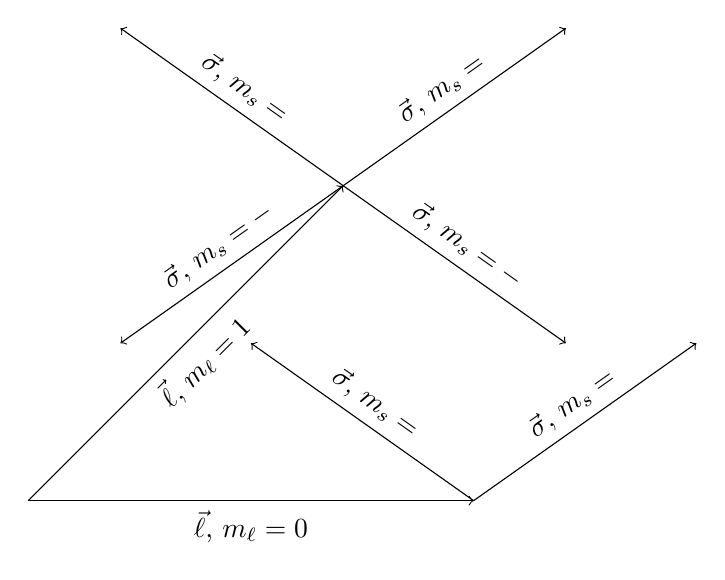
\begin{tikzpicture}[scale=4]
		\coordinate (l1) at (45:1.41421);
		\coordinate (l0) at (0:1.41421);
		\coordinate (l-1) at (-45:1.41421);

		\coordinate (s+l) at (144.736:0.866025);
		\coordinate (s+r) at (35.2644:0.866025);
		\coordinate (s-l) at (-144.736:0.866025);
		\coordinate (s-r) at (-35.2644:0.866025);

		\draw[->] (0, 0) -- (l1) node[midway, sloped, below] {$\vec \ell$, $m_\ell=1$};
		\draw[->] (0, 0) -- (l0) node[midway, sloped, below] {$\vec \ell$, $m_\ell=0$};

		\draw[->] (l0) -- ($(l0)+(s+r)$) node[midway, sloped, above] {$\vec \sigma$, $m_s=\half$};
		\draw[->] (l0) -- ($(l0)+(s+l)$) node[midway, sloped, above] {$\vec \sigma$, $m_s=\half$};
		\draw[->] (l1) -- ($(l1)+(s+r)$) node[midway, sloped, above] {$\vec \sigma$, $m_s=\half$};
		\draw[->] (l1) -- ($(l1)+(s+l)$) node[midway, sloped, above] {$\vec \sigma$, $m_s=\half$};

		\draw[->] (l1) -- ($(l1)+(s-r)$) node[midway, sloped, above] {$\vec \sigma$, $m_s=-\half$};
		\draw[->] (l1) -- ($(l1)+(s-l)$) node[midway, sloped, above] {$\vec \sigma$, $m_s=-\half$};
	\end{tikzpicture}
	\caption{%
		Alle Vektoren $\vec l$ und $\vec \sigma$ in einem Diagramm. Dabei habe
		ich die Fälle, in denen alle $z$-Komponenten umgekehrt sind,
		weggelassen, da sie letztlich das gleiche darstellen.
	}
	\label{fig:4/a/alle}
\end{figure}

\begin{figure}
	\centering
	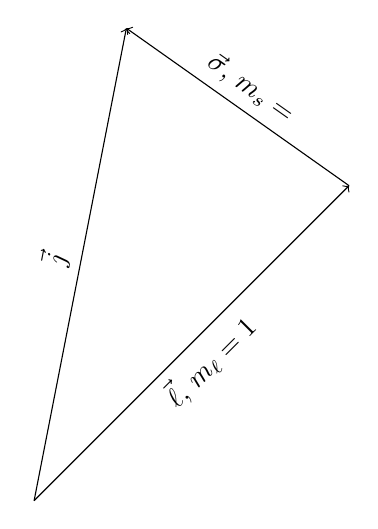
\begin{tikzpicture}[scale=4]
		\coordinate (l1) at (45:1.41421);
		\coordinate (l0) at (0:1.41421);
		\coordinate (l-1) at (-45:1.41421);

		\coordinate (s+l) at (144.736:0.866025);
		\coordinate (s+r) at (35.2644:0.866025);
		\coordinate (s-l) at (-144.736:0.866025);
		\coordinate (s-r) at (-35.2644:0.866025);

		\draw[->] (0, 0) -- (l1) node[midway, sloped, below] {$\vec \ell$, $m_\ell=1$};
		\draw[->] (l1) -- ($(l1)+(s+l)$) node[midway, sloped, above] {$\vec \sigma$, $m_s=\half$};
		\draw[->] (0, 0) -- ($(l1)+(s+l)$) node[midway, sloped, above] {$\vec j$};
	\end{tikzpicture}
	\caption{%
		$m_\ell = 1$ und $m_s = \half$
	}
	\label{fig:4/a/1}
\end{figure}

\begin{figure}
	\centering
	\begin{tikzpicture}[scale=4]
		\coordinate (l1) at (45:1.41421);
		\coordinate (l0) at (0:1.41421);
		\coordinate (l-1) at (-45:1.41421);

		\coordinate (s+l) at (144.736:0.866025);
		\coordinate (s+r) at (35.2644:0.866025);
		\coordinate (s-l) at (-144.736:0.866025);
		\coordinate (s-r) at (-35.2644:0.866025);

		\draw[->] (0, 0) -- (l1) node[midway, sloped, above] {$\vec \ell$, $m_\ell=1$};
		\draw[->] (l1) -- ($(l1)+(s+r)$) node[midway, sloped, above] {$\vec \sigma$, $m_s=\half$};
		\draw[->] (0, 0) -- ($(l1)+(s+r)$) node[midway, sloped, below] {$\vec j$};
	\end{tikzpicture}
	\caption{%
		$m_\ell = 1$ und $m_s = \half$
	}
	\label{fig:4/a/2}
\end{figure}

\begin{figure}
	\centering
	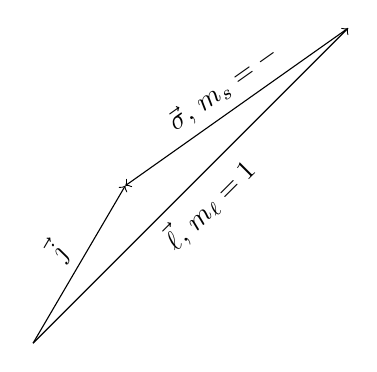
\begin{tikzpicture}[scale=4]
		\coordinate (l1) at (45:1.41421);
		\coordinate (l0) at (0:1.41421);
		\coordinate (l-1) at (-45:1.41421);

		\coordinate (s+l) at (144.736:0.866025);
		\coordinate (s+r) at (35.2644:0.866025);
		\coordinate (s-l) at (-144.736:0.866025);
		\coordinate (s-r) at (-35.2644:0.866025);

		\draw[->] (0, 0) -- (l1) node[midway, sloped, below] {$\vec \ell$, $m_\ell=1$};
		\draw[->] (l1) -- ($(l1)+(s-l)$) node[midway, sloped, above] {$\vec \sigma$, $m_s=-\half$};
		\draw[->] (0, 0) -- ($(l1)+(s-l)$) node[midway, sloped, above] {$\vec j$};
	\end{tikzpicture}
	\caption{%
		$m_\ell = 1$ und $m_s = -\half$
	}
	\label{fig:4/a/3}
\end{figure}

\begin{figure}
	\centering
	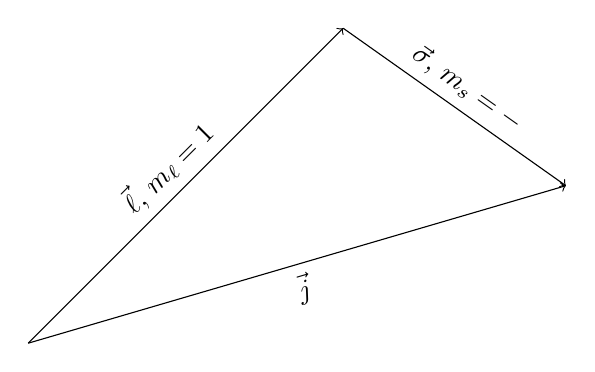
\begin{tikzpicture}[scale=4]
		\coordinate (l1) at (45:1.41421);
		\coordinate (l0) at (0:1.41421);
		\coordinate (l-1) at (-45:1.41421);

		\coordinate (s+l) at (144.736:0.866025);
		\coordinate (s+r) at (35.2644:0.866025);
		\coordinate (s-l) at (-144.736:0.866025);
		\coordinate (s-r) at (-35.2644:0.866025);

		\draw[->] (0, 0) -- (l1) node[midway, sloped, above] {$\vec \ell$, $m_\ell=1$};
		\draw[->] (l1) -- ($(l1)+(s-r)$) node[midway, sloped, above] {$\vec \sigma$, $m_s=-\half$};
		\draw[->] (0, 0) -- ($(l1)+(s-r)$) node[midway, sloped, below] {$\vec j$};
	\end{tikzpicture}
	\caption{%
		$m_\ell = 1$ und $m_s = -\half$
	}
	\label{fig:4/a/4}
\end{figure}

\begin{figure}
	\centering
	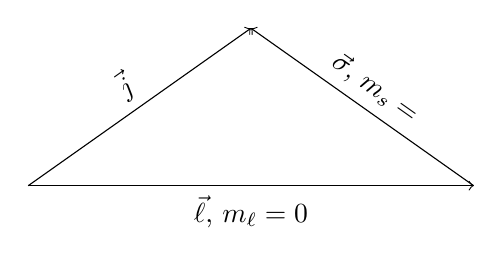
\begin{tikzpicture}[scale=4]
		\coordinate (l1) at (45:1.41421);
		\coordinate (l0) at (0:1.41421);
		\coordinate (l-1) at (-45:1.41421);

		\coordinate (s+l) at (144.736:0.866025);
		\coordinate (s+r) at (35.2644:0.866025);
		\coordinate (s-l) at (-144.736:0.866025);
		\coordinate (s-r) at (-35.2644:0.866025);

		\draw[->] (0, 0) -- (l0) node[midway, sloped, below] {$\vec \ell$, $m_\ell=0$};
		\draw[->] (l0) -- ($(l0)+(s+l)$) node[midway, sloped, above] {$\vec \sigma$, $m_s=\half$};
		\draw[->] (0, 0) -- ($(l0)+(s+l)$) node[midway, sloped, above] {$\vec j$};
	\end{tikzpicture}
	\caption{%
		$m_\ell = 0$ und $m_s = \half$
	}
	\label{fig:4/a/5}
\end{figure}

\begin{figure}
	\centering
	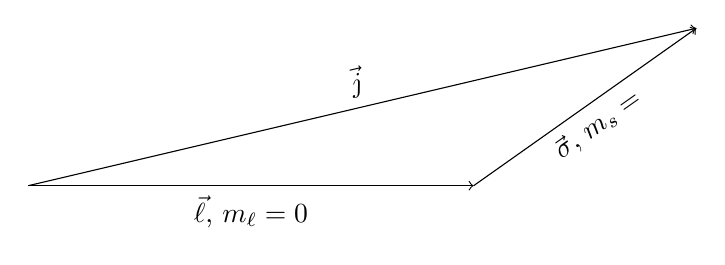
\begin{tikzpicture}[scale=4]
		\coordinate (l1) at (45:1.41421);
		\coordinate (l0) at (0:1.41421);
		\coordinate (l-1) at (-45:1.41421);

		\coordinate (s+l) at (144.736:0.866025);
		\coordinate (s+r) at (35.2644:0.866025);
		\coordinate (s-l) at (-144.736:0.866025);
		\coordinate (s-r) at (-35.2644:0.866025);

		\draw[->] (0, 0) -- (l0) node[midway, sloped, below] {$\vec \ell$, $m_\ell=0$};
		\draw[->] (l0) -- ($(l0)+(s+r)$) node[midway, sloped, below] {$\vec \sigma$, $m_s=\half$};
		\draw[->] (0, 0) -- ($(l0)+(s+r)$) node[midway, sloped, above] {$\vec j$};
	\end{tikzpicture}
	\caption{%
		$m_\ell = 0$ und $m_s = \half$
	}
	\label{fig:4/a/6}
\end{figure}

\subsection{Magnetische Momente}

Für die magnetischen Momente gilt:
\[
	\vec \mu_\ell = - \mu_B \vec \ell
	\eqnsep
	\vec \mu_s = - 2 \mu_B \vec \sigma
\]

Das magnetische Moment des Spins ist also im Vergleich zu den Drehmomenten
doppelt so groß wie das magnetische Moment des Spins. Daher ist die vektorielle
Summe $\vec \mu_j$ auch anders als $\vec j$.

In Abbildung \ref{fig:4/a/1} habe ich die magnetischen Momente eingetragen, das
Resultat ist in Abbildung \ref{fig:4/b/1}.

\begin{figure}
	\centering
	\begin{tikzpicture}[scale=4]
		\coordinate (l1) at (45:1.41421);
		\coordinate (l0) at (0:1.41421);
		\coordinate (l-1) at (-45:1.41421);

		\coordinate (mul1) at (l1);

		\coordinate (s+l) at (144.736:0.866025);
		\coordinate (s+r) at (35.2644:0.866025);
		\coordinate (s-l) at (-144.736:0.866025);
		\coordinate (s-r) at (-35.2644:0.866025);

		\coordinate (mus+l) at (144.736:1.73205);

		\draw[->, dotted] (0, 0) -- (l1) node[midway, sloped, below] {};
		\draw[->, dotted] (l1) -- ($(l1)+(s+l)$) node[midway, sloped, above] {};
		\draw[->] (0, 0) -- ($(l1)+(s+l)$) node[midway, sloped, above] {$\vec j$};

		\draw[->] (0, 0) -- (mul1) node[midway, sloped, below] {$\vec \mu_\ell$};
		\draw[->] (mul1) -- ($(mul1)+(mus+l)$) node[midway, sloped, above] {$\vec \mu_s$};
		\draw[->] (0, 0) -- ($(mul1)+(mus+l)$) node[midway, sloped, above] {$\vec \mu_j$};
	\end{tikzpicture}
	\caption{%
		$m_\ell = 1$ und $m_s = \half$
	}
	\label{fig:4/b/1}
\end{figure}

In dieser Abbildung ist dann auch zu sehen, dass $\vec j \nparallel \vec\mu_j$
gilt.

\subsection{Präzession von $\vec \mu_j$ um $\vec j$}

\fehlt

\subsection{$g$-Faktoren}

\fehlt

\subsection{externes Magnetfeld}

\fehlt

%%%%%%%%%%%%%%%%%%%%%%%%%%%%%%%%%%%%%%%%%%%%%%%%%%%%%%%%%%%%%%%%%%%%%%%%%%%%%%%
%                                    Ende                                     %
%%%%%%%%%%%%%%%%%%%%%%%%%%%%%%%%%%%%%%%%%%%%%%%%%%%%%%%%%%%%%%%%%%%%%%%%%%%%%%%

\IfFileExists{\bibliographyfile}{
	%\bibliography{\bibliographyfile}
}{}

\end{document}

% vim: spell spelllang=de
